%% Copyright 1998 Pepe Kubon
%%
%% `two.tex' --- 2nd chapter for thes-full.tex, thes-short-tex from
%%               the `csthesis' bundle
%%
%% You are allowed to distribute this file together with all files
%% mentioned in READ.ME.
%%
%% You are not allowed to modify its contents.
%%

%%%%%%%%%%%%%%%%%%%%%%%%%%%%%%%%%%%%%%%%%%%%%%%%%
%
%     Chapter 2   
%
%%%%%%%%%%%%%%%%%%%%%%%%%%%%%%%%%%%%%%%%%%%%%%%%

\chapter{Literature Review}
\label{chap:two}
This chapter provides a literature review of the state-of-the-art methods in the field of outlier detection. 
%In Section \ref{sec:outdefinition}, we formally define outlier, different types of outlier and the applications of outlier detection. 
Outlier detection is a very well-explored area and there are many surveys to overview the state-of-the-art methods. Each survey categorized these methods differently. The categorization can be based on datatype (e.g. graph data) or type of methods that have been used to detect outliers (e.g. structured-based methods). In this chapter we group outlier methods based on the format of the input data, whether it is presented in a single data table or it has a higher level of organization such as data presented in a relational database, or XML format or OLAP. Since the focus of our work is on the structured data, we mainly concentrate on the methods designed for that data format .\\% We further categorized each type into supervised and unsupervised approaches. 
%Different surveys categorized outlier detection work In Section \ref{sec:categorizedMethods}, we categorized different outlier detection techniques into supervised and unsupervised and briefly discuss some methods of each category.
% Since the focus of this dissertation is on outlier detection for Object-relational data, we devote the entire Section \ref{sec:outlierinSRL} to explore relational-based outlier detection methods. 
 We conclude this chapter with section \ref{sec:limitaion} which addresses the limitations of current outlier detection methods. Figure~\ref{fig:categorization} shows the organization of this chapter.
	\begin{figure*}[!htbp]
		\centering
		\resizebox{0.8\textwidth}{!}{
			\includegraphics%[width=0.3\textwidth] 
			{figures/chapt2Category.pdf}
		}
		\caption{ Related work categorization
			\label{fig:categorization}}
	\end{figure*}
%\section{Background and Notation \label{sec:background}}
%In this section, we introduce some	notation and terminology that is referred to throughout this dissertation. We present a brief discussion on probability, Bayesian networks and Markov Logic Network. Please refer to the citations to find more information for any of the discussed topics.
%
%\subsection{Probability Distribution}
% Throughout this dissertation, \textbf{random variables} are denoted by  by capital letters (X,Y,...) and the values of a random variable by lower case letters (x,y,...).  We denote sets of random variables by \textbf{X}=\{$\X_{1},\ldots,\X_{n}$\}. 
%%The \textbf{range} of the variable is the set of values of the variable. In this dissertation we only consider random variables with a \emph{finite range}.
% The notation $P(X_1 = x_1,...,X_n = x_n) = p$, sometimes abbreviated as $P(\x_1,...,\x_n) = p$, or $P(\mathbf{X} = \mathbf{x}) = p$ means that the \textbf{joint probability} of random variables $X_{1},\ldots,X_{n}$ taking on values $\x_1,\dots,\x_n$ is $p$. 
% 
%By the laws of probability the sum of the joint probability distribution of a set of random variables $\textbf{\X}$ over all possible values $\textbf{x}$ is 1, that is,
%
%$$\sum_\textbf{x}{ P(\textbf{X} =\textbf{x})}=1 $$  
%
%
%The joint probability distribution of a subset $\textbf{Y}$ of $\textbf{X}$ can be obtained by summing out the remaining variables $\textbf{Z} = \textbf{X} \backslash \textbf{Y}$. The distribution is called the \textbf{marginal probability} distribution of $\textbf{\Y}$ and can be obtained by the following formula:
%
%$$ P(\textbf{Y}) = \sum_{\textbf{z}} P(\textbf{Y}, \textbf{Z} = \textbf{z}) $$
%
%Given as subset  $\textbf{Z} \in \textbf(Z)$, the \textbf{conditional probability} of a subset  $\textbf(Y) \in \textbf(X)$ can be derived from the following formula:
%$$ P(\textbf{Y}| \textbf{Z}) = \frac{P(\textbf{Y}, \textbf{Z})}{P(\textbf{Z})}$$
%
%%The conditional probability of a subset $\textbf(Y) \in \textbf(X)$ given a subset $\textbf{Z} \in \textbf(Z)$ is the probability of  $\textbf{Y}$ occurring when we know $\textbf{Z}$ has occurred. The \textbf{conditional probability} can be obtained by the following formula:
%%
% \emph{Independent} events are events that occurrence of one event does not effect the other. The joint probability of the two independent  events is the product of each event occurrence. 
%%
%%Two events $\textbf{X}$ and $\textbf{Y}$ are \emph{independent} if occurrence of  $\textbf{X}$ does not effect the probability of $\textbf{Y}$ occurring. In such a event, the joint probability of the two events co-occurring is calculated by the product of each of their occurrence:
%
%$$ P(\textbf{X}, \textbf{Y}) = P(\textbf{X}) \times P(\textbf{Y})$$
%
%\subsection{Predicate Language}
%
%We employ the notation of Chiang and Poole \cite{Chiang2012} for logical syntax, as follows.
%%
%Constants are expressed in lower-case, e.g. $\it{joe}$, and are used to represent individuals. A type is associated with each individual, e.g. $\it{joe}$ is a person. We use $D(\tau)$ to represent a domain of type $\tau$, which is the set of individuals of type $\tau$. A {\em logical variable} is written in upper case. A logical variable is also typed, e.g. $\it{Person}$ denotes some member of $D(\tau)$. A relation is given by 
%$$r : \Omega \rightarrow V_{r}$$
%where $r$ is the name of the relation, $\Omega_{r}=D(\tau_{1})\times \ldots \times D(\tau_{a})$ is the domain of the relation, and $T_{r}=(\tau_{1},\ldots,\tau_{a})$ is the type of the relation. $V_{r}={v_{1},\ldots,v_{k}}$ is the range of the relation. Number $a$ and $k$ are positive integers denoting the {\em arity} and {\em size} of $r$. An {\em atom} is an expression of the form $r(\sigma_{1},\ldots,\sigma_{a})$ where each $\sigma_{i}$ is either a constant or logical variable. If all of $\sigma_{1},\ldots,\sigma_{a}$ are constants, $r(\sigma_{1},\ldots,\sigma_{a})$ is a {\em ground atom}.
%
%A {\em literal} specifies the value of an atom e.g. $r(X_{1},\ldots,X_{a})=v$ where $v \in V_{r}$. A literal is also a {\em formula}. Formula with multiple literals are formed using connectives $\wedge$ and or $\vee$. Connecting literals using only $\wedge$ forms a {\em conjunctive formula } or {\em conjunction}. A formula that contains no logical variables is a {\em ground} formula.
%%, is a proposition.
%%A {\em disjunctive formula} or {\em disjunction} is formed using only $\vee$. \\
%
%A substitution is a set $\{X_{1} \textbackslash x_{1}, \ldots, X_{k}\textbackslash x_{k}\}$ where $X_{i}$ are distinct logical variables and $x_{i}$ are constants. When applied to a formula $f$, each occurrence of $X_{i}$ in $f$ is replaced with $x_{i}$. We denote the application of a substitution 
%%$\{X_{1} \textbackslash x_{1}, \ldots, X_{k}\textbackslash x_{k}\}$ 
%to $f$ as $f\{X_{1} \textbackslash x_{1}, \ldots, X_{k}\textbackslash x_{k}\}$. 
%Consider a formula $f$ containing logical variables $X_{1}, \ldots,X_{n}$, where each $X_{i}$ has type $\tau_{i}$. The {\em grounding space} of $f$, is the set of all possible grounding substitutions for $f$, given by 
%$$\{\{X_{1}\textbackslash x_{1}, \ldots, X_{n}\textbackslash x_{n}\}:x_{i} \in D(\tau_{i}) \mbox{ for } i=1,\ldots,n\}.$$
%
%%	Given some formula $f$ containing logical variables $X_{1}, \ldots,X_{n}$, where each $X_{i}$ has type $\tau_{i}$, let the domain of $f$ be $\Omega_{f}=D(\tau_{i}\times \tau_{n})$. The {\em substitution space} of $f$, $\Gamma_{f}$, is the set of all possible grounding substitutions for $f$, given by 
%%	$$\Gamma_{f}=\{\{X_{1}\textbackslash x_{1}, \ldots, X_{n}\textbackslash x_{n}\}:(x_{1},\ldots,x_{n})\in \Omega_{f}\}.$$
%
%A \emph{database} $\D$ specifies for each ground literal whether the literal is true in the database or not. A ground conjunction is true in a database if all of its conjuncts are true. The \emph{count} of groundings satisfying formula $\formula$ with respect to a database $\D$ is denoted as $\grounds_{\D}(\formula)$.
%
%\subsubsection{Examples} Figure~\ref{fig:exampledatabase} shows an example database. The ground literal $$(\it{ShotEff(\P,\M)} = Low) \{\P\textbackslash 123,\M\textbackslash 1\}=(\it{ShotEff}(123,1)=Low)$$ evaluates as true in this database. For the grounding count we have $$\grounds_{\D}(\it{ShotEff(\P,\M)} = Low) \{\P\textbackslash 123\}) = 2.$$
%
%
%
%\begin{figure*}[htbp]
%	\centering
%	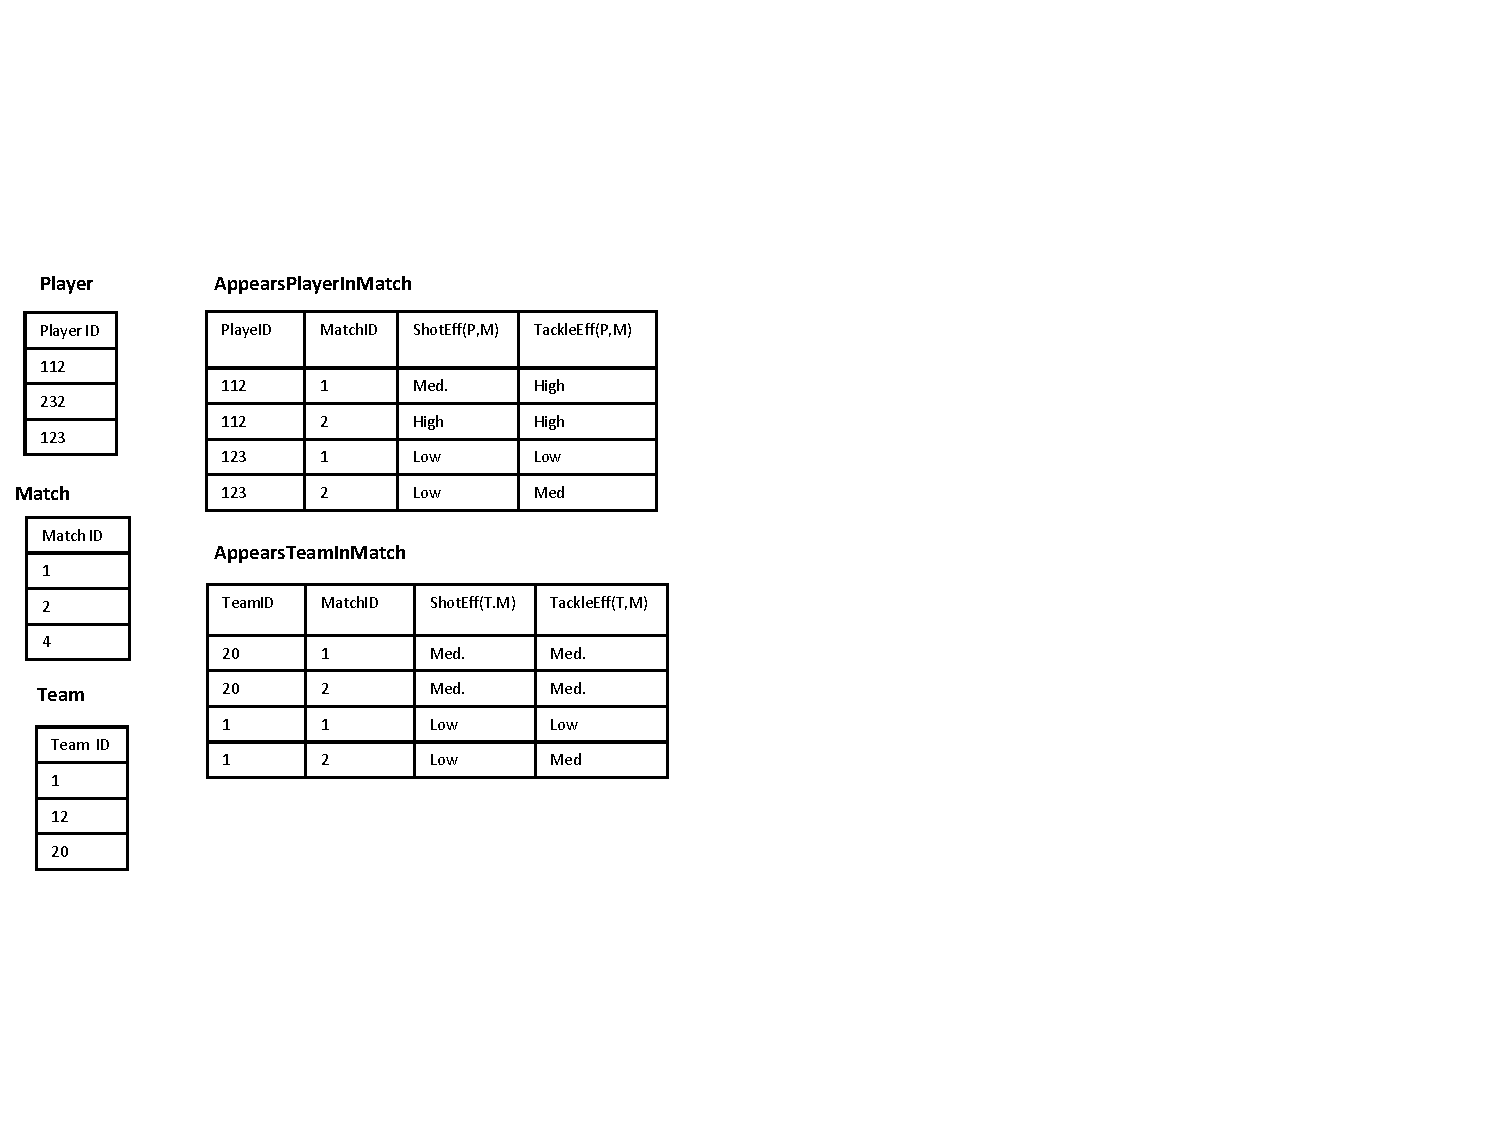
\includegraphics[width=0.5\textwidth]{figures/databasefigure.pdf}
%	\caption{An example database
%		\label{fig:exampledatabase}}
%\end{figure*}
%\subsection{Bayesian Networks} \label{Sec:BayesianNetwork}
%A {\bf Bayesian Network (BN)} is a directed acyclic graph (DAG) whose nodes comprise a set of random variables \cite{Pearl1988}. Depending on context, we interchangeably refer to the nodes  and variables of a BN. Fix a set of variables $\Features = \{\feature_{1},\ldots,\feature_{n}\}$. 
%%These are attributes of objects, which can and typically do belong to different classes. In statistical terms, each attribute defines a random variable. 
%The possible values of $\feature_{i}$ are enumerated as $\{\nodevalue_{i1},\ldots,\nodevalue_{i\states_{i}}\}$. The notation $P(\feature_{i} = \nodevalue)\equiv P(\nodevalue)$ denotes the probability of variable $\feature_{i}$ taking on value $\nodevalue$. We also use the vector notation $P(\Features = \set{\nodevalue}) \equiv P(\set{\nodevalue})$ to denote the joint probability that each variable $\feature_{i}$ takes on value $\set{\nodevalue}_{i}$. 
%
%
%The conditional probability parameters of a Bayesian network specify the distribution of a child node given an assignment of values to its parent node. For an assignment of values to its nodes, a BN defines the joint probability as the product of the conditional probability of the child given its parent values, for each child node in the network. This means that the log-joint probability can be {\em decomposed} as the node-wise sum
%
%\begin{equation} \label{eq:bn}
%\ln P(\Features = \set{\nodevalue};\model,\parameters) = \sum_{i=1}^{n} \ln \parameter(\set{\nodevalue}_{i}|\set{\nodevalue}_{\parents_{i}})
%\end{equation}
%
%where $\set{\nodevalue}_{i}$ resp. $\set{\nodevalue}_{\parents_{i}}$ is the assignment of values to node $i$ resp. the parents of $i$ determined by the assignment $\set{\nodevalue}$. 
%%The function $\ln$ is the binary logarithm base 2. 
%To avoid difficulties with $\ln(0)$, here and below we assume that joint distributions are positive everywhere. Since the parameter values for a Bayes net define a joint distribution over its nodes, they therefore entail a marginal, or unconditional, probability for a single node. We denote the \textbf{marginal probability} that node $\feature$ has value $\nodevalue$ as $P(\feature = \nodevalue;\model,\parameters) \equiv \parameter(\nodevalue)$.
%
%\paragraph{Example.} Figure~\ref{fig:BayesNet} shows an example of a Bayesian network and associated joint and marginal probabilities.
%\begin{figure} %  figure placement: here, top, bottom, or page
%	\centering
%	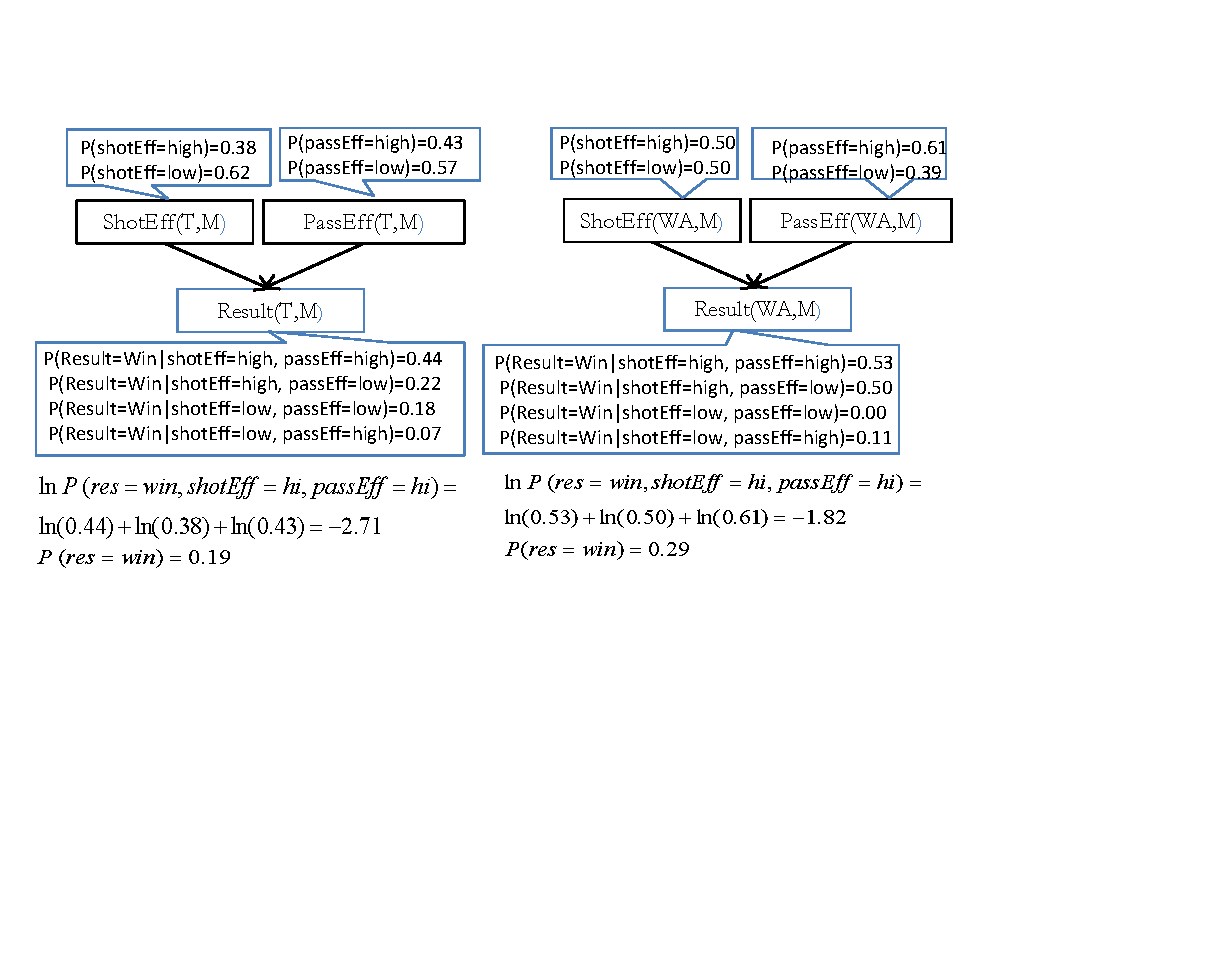
\includegraphics[width=0.9\textwidth]{figures/bnuncropped} 
%	\caption [An example of a Bayesian network ]{ Example of joint and marginal probabilities computed from a toy Bayesian Network structure \label{fig:BayesNet}}
%\end{figure}
%\subsubsection{Learning Bayesian Networks} \label{Sec:learningBN}
%The goal of structure learning is to find a directed acyclic graph $G$ that represents a set of variables $V$ and a dataset $\mathcal{D}$ containing independent and identically distributed (i.i.d) examples from an unknown distribution $P$. For every possible edge in the network structure leaning algorithm must determine whether to include that in the final network or not. The total possible number of graphs is super exponential in $|V|$. Even restricting the domain and constraining variables to have at most $k$ parents has been proven to be NP-Complete.
%\subsubsection{Markov Logic Network} \label{Sec:MLNIntro}
%Markov Logic Network~\cite{Domingos07} 
%is one of the most well known methods of statistical relational learning. Essentially an MLN consists of a set of weighted first-order formulas that defines a Markov network comprising ground instances of logical predicates. The formulas are the structure of the network and represent associations between ground facts. The weights are the parameters of quantitative components and assign a likelihood to a given relational database by using the log-linear formalism of Markov networks. Table~\ref{MLNSample} shows an MLN for the Soccer domain.
%
%%\begin{table} 
%%	\caption{Example of a small MLN}
%%	\centering
%%	\resizebox{0.9\textwidth}{!}{
%%		\begin{tabular}{|c|c|l|}
%%			\hline
%%			First-order logic formula&Weight&Translation\\\hline
%%			$\forall(shotEfficiency(p)\rightarrow dribbleEfficiency(p))$&$w_{1}$&
%%			\begin{tabular}{p{3cm}} if shot efficiency of the player is high\\, dribble efficiency is high \end{tabular}\\\hline
%%			
%%			%Synthetic&40&280\\ \hline
%%		\end{tabular}}\label{MLNSample}
%%	\end{table}
%\begin{table}
%	\centering
%	\begin{tabular}
%		{|l|l|l|} \hline
%		First-order logic  & Weight& English \\ \hline
%		\multirow{2}{*} {$\forall x (shotEfficiency(x) \Rightarrow dribbleEfficiency(x))  $} & \multirow{2}{*} {$w_1$} & if shot efficiency of the player is \\ & &high then  dribble efficiency is high \\ \hline
%%		$\forall x \forall y (intelligent(x) \wedge  friend(x,y)$ & \multirow{2}{*}{ 0.7}& If a student has an intelligent \\ $\Rightarrow$ $intelligent(y)$) & & friend then he is intelligent  \\ \hline
%	\end{tabular}
%	\caption{Example of a small MLN }
%	\label{MLNSample}
%\end{table}
%Given a set of variables $V$ and a dataset $\mathcal{D}$ containing independent and identically distributed (i.i.d) examples from an unknown distribution $P$, the goal of structure learning is to identify a directed acyclic graph $G$ that represents $P$.
% Finding an optimal structure is a computationally intractable problem; structure learning algorithms determine for every possible edge in the network whether or not to include the edge in the final network and which direction to orient the edge. The total possible number of graphs is super exponential in $|V|$. Even a restricted form of structure learning where variables are constrained to have at most $k$ parents has been proven to be NP-Complete.
% Two broad classes of structure learning are well-known in the literature \cite{Neapolitan2004,Heckerman1998}. 
%
%\begin{itemize}
%	\item Score Based methods search over possible Bayesian network structures for the most suitable factorization of the joint probability based on $\mathcal{D}$. The model selection criterion is usually defined as a score that the methods are trying to maximize. BDeu \cite{Heckerman1994} and BIC \cite{Chickering2003} are examples of well known scores for Bayesian network learning.
%	
%	\item Constraint Based methods employ a statistical tests to detect conditional (in)dependencies given a sample $\mathcal{D}$, and then compute a BN structure $G$ that fits the (in)dependencies \cite{Margaritis2000,Cheng2002}. The  (in)dependencies test can be chosen to suit the type of available data and application domain. One of the traditional test for categorical data is the $\chi^2$ test.
%
%\end{itemize}
%
%To form a complete Bayes net, an additional step of parameter estimation is required to determine ${\theta}_G$ from $\mathcal{D}$. Since the focus of this dissertation is on structure learning, techniques for parameter estimation will not be addressed here. (See e.g. \cite{Heckerman1998} for details).

%\subsubsection{Parametrized  Bayes Nets}
%Parametrized Bayes nets(PBNs) were introduced by Poole to study first-order probabilistic inference on directed models. They are a comparatively simple adaptation of the Bayes net format for relational data. The syntax of PBNs is similar to that of other directed graphical SRL models, such as Bayes Logic Programs \cite{Kersting2007} and Probabilistic Graphical Models \cite{Friedman99prm}. A Parametrized Bayes Net structure consists of: (1) a directed acyclic graph whose nodes are functor nodes. (2) a population for each first-order variable. (3) an assignment of a range to each functor. A Parametrized Bayes Net is a Bayes net whose graph is a  parametrized Bayes Net structure. Because each of the nodes in a parametrized Bayes net is a functor, We also use the name Functor Bayes Nets (FBNs) for them. 


%\subsection{Relational Data and Databases} \label{sec:relationaldata}
% We adopt a functor-based notation for combining logical and statistical concepts~\cite{Poole2003,Kimmig2014}.
% A functor is a function or predicate symbol. Each functor has a set of values (constants) called the \textbf{domain} of the functor. The domain of a \textbf{predicate} is $\{\true,\false\}$. Predicates are usually written with uppercase Roman letters, other terms with lowercase letters.
% A predicate of arity at least two is a \textbf{relationship} functor. Relationship functors specify which objects are linked. Other functors represent \textbf{features} or \textbf{attributes} of an object or a tuple of objects (i.e., of a relationship).
% A \textbf{population} is a set of objects. 
% A \textbf{term} is of the form $f(\term_{1},\ldots,\term_{k})$ where $\functor$ is a functor %(either a function symbol or a predicate symbol) 
% and each $\term_{i}$ is a first-order variable or a constant denoting an object. A term is \textbf{ground} if it contains no first-order variables; otherwise it is a first-order term. In the context of a statistical model, we refer to first-order terms as \textbf{Parametrized Random Variables} (PRVs) \cite{Kimmig2014}. 
% %A term whose range are the truth values $\{\true,\false\}$ is a \textbf{predicate}. 
% %Predicates are usually written with uppercase Roman letters, other term with lowercase letters.
% %The grounding concept represents moving from the population-level  to the object level. 
% A \textbf{grounding} replaces each first-order variable in a term by a constant; the result is a ground term. A grounding may be applied simultaneously to a set of terms.  A relational database $\D$ specifies the values of all ground terms, which can be listed in data tables. 
% %In machine learning terminology, the data tables are contingency tables that represent sufficient statistics or event counts.
 
% Consider a joint assignment 
% $P(\Features = \set{\nodevalue})$ of values to a set of PRVs $\Features$. The {\em grounding space} of the PRVs is the set of all possible grounding substitutions, each applied to all PRVs in $\Features$. The {\em count} of groundings that satisfy the assignment with respect to a database $\D$ is denoted by $\grounds_{\D}(\Features = \set{\nodevalue})$. The \textbf{database frequency} $P_{\D}(\Features = \set{\nodevalue})$ is the grounding count divided by the number of all possible groundings.
% 

%\paragraph{Object-relational data}
%\subsection{Object-relational data} \label{Sec:objectRelationl}

\section{Outlier Detection Methods for Propositional Data} \label{sec:categorizedMethods}
In this section we explore outlier detection methods that take \textit{propositional} data. One interpretation of propositional data is that the attributes describe characteristics of one object-class. For example, $\mathit{shotEfficiency(Player)}$ shows shot efficiency of a player in general, while in the structured data the attributes are more complex; for example in the Object-relational data model, the attributes are shown in this format: $\mathit{shotEfficiency(Player, Match})$ which represents shot efficiency of a player in a match and involves two object-classes.   Throughout this dissertation, we call the methods designed for single data table propositional methods. In this section, we further categorize these methods into supervised and unsupervised based on whether the sample of data has been provided with labels and domain expert information to build an outlier detection model.
%\begin{figure*}[!htbp]
%	\centering
%	\resizebox{1\textwidth}{!}{
%		\includegraphics%[width=0.3\textwidth] 
%		{figures/structure.pdf}
%	}
%	\caption{Categorizing outlier detection methods.
%		\label{fig:Overview}}
%\end{figure*}
\subsection{Supervised Methods for Propositional Data}
These methods model both normality and abnormality and requires pre-labelled data. Normal points may belong to a single class or be divided among different classes. Supervised outlier detection is a special case of the classification where the labels are extremely unbalanced in terms of occurrence~\cite{Chawla2004}.
Normal data points are easily available while outlier examples are very sparse and it is the rarity that makes these data points outliers. In this sense, outlier detection can also be viewed as $\it{rare class}$ detection problem. The imbalanced nature of outlier detection makes the accurate classifications quite hard to achieve and it might result in over-training \cite{aggarwal2013}.

When the purpose of classification is outlier detection, cost-sensitive variations of machine learning algorithms can be used in order to make the classification of anomalies more accurate \cite{aggarwal2013}.
Class imbalance is one of the common problems in supervised outlier detection. The standard evaluation techniques in classifications cannot simply be applied to outlier detection. For example, in the case of breast cancer, where 99\% of scans are identified to be normal and only 1\% abnormal, the trivial classification algorithm, which returns all the instances in the test cases as normal, would have a high accuracy of 99\%. However, it is not useful in the context of detecting breast cancer. Cost-sensitive learning is one way that has been used to handle the class imbalance problem in outlier detection. The objective function of the classification in this type of learning has been designed in a way that it weights the errors in classification differently for different classes.  In this case, classifiers are tuned so the errors in classification of outliers are more penalized compared to the misclassified normal classes~\cite{Elkan2001}. In other words, methods are forced to predict the outlier class far better than the normal class. This trade-off is characterized either by the precision-recall curve or a receiver operating characteristics ($ROC$) curve.\\
Active re-sampling is another way to tackle class imbalance problem. The relative proportion of the rare classes is magnified through re-sampling. This approach can be considered as an indirect form of cost-sensitive learning.\\
Classification outlier methods can be grouped into two categories: 
\begin{itemize}
	\item Multi-class: Training data in this group contains the instances from multiple normal classes~\cite{Claudio2000}. First, a classifier is learned to distinguish between instances from different normal classes. If a test instance is not classified as normal by any of the classifiers, then it is labeled as an outlier.
	\item One-class: All training instances belong to a single class label. If any test case does not fall into the normal boundary, it is identified as an outlier. Examples of well-known algorithms are:
	\begin{itemize}
		\item  One-class SVMs \cite{Scholkopf2001}
		\item  One-class Kernel Fisher Discriminant~\cite{Roth2005}
	\end{itemize}
\end{itemize}


In the following subsections, we provide examples of supervised methods in different areas.

%\subsubsection{Naive Baye}
%Naive Bayesian networks for classifications can also be applied to outlier detection. Amor {\em et al.}  uses Naive Bayes in intrusion detection and consider three levels of attack~\cite{Amor2004}: 
%\begin{enumerate}
%	
%	
%	\item Whole attacks where they evaluate the ability of Naive Bayes to detect each elementary attack.
%	\item Group the attacks into four main categories to identify which category a given connection belongs to.
%	\item Focus on normal and abnormal behavior and estimate whether an observation falls into one class or not.
%\end{enumerate}

% \cite{Das2008} focuses on detecting anomalies in categorical datasets.

\subsubsection{Neural Network}
Neural networks are applied to outlier detection in one-class learning as well as multi-class  scenarios. At the first step, a neural network is trained on normal training data in order to learn the normal behavior of data points. Then, test instances are presented to the neural network. If the test is accepted, the data point is normal, otherwise, it is an outlier. Different neural network techniques have been proposed to tackle outlier detection problem. Ghosh {\em et al.} \cite{Ghosh98} apply multi-layered perceptrons and focus on detecting attacks on computer systems. They perform intrusion detection on software programs instead of what most intrusion detection systems do by analyzing network traffic and host system logs. They build a profile of software behaviour to distinguish between a normal software behaviour and a malicious one.

\subsubsection{Support Vector Machine}
Support Vector Machines have been applied to outlier detection mostly in a one-class setting. These techniques first learn a region that includes the training data points. If a test instance falls into the learned region, it is considered as normal, otherwise, it is an outlier~\cite{DavyG02,RatMikSchMul02}.
%\subsubsection{Hidden Markov Model}
%Zhang {\em et al.}~\cite{Zhang2005} designed a semi-supervised hidden markov model framework that learns normal events from labeled samples and unusual events are modeled using Maximum a Posteriori adaptation. By maximizing the likelihood of observation sequences of the normal events, a set of parameters of {\em HMM} models is learned. The probability density function of the learned model is assumed to be Gaussian mixture model. Given this well estimated normal event model, the likelihood of each test data point is computed. 
\subsection{Unsupervised Methods for Propositional Data}
In the datasets where data points are not labeled, unsupervised approaches make some assumptions about the behaviour of outliers. Based on the assumptions made, these methods can be categorized.
\subsubsection{Probabilistic and Statistical Models}
In the probabilistic and statistical model, the data is assumed to be derived from a closed form of probability distribution and the goal is to learn the parameters of this model. Therefore, the main challenge is to choose the data distribution. The parameter of the distribution can be learned by using different algorithms, such as Expectation Maximization. The key output of this method is the membership probability of data points to the distribution; the ones that have a very low fit will be considered as outliers. Extreme Value Test can also determine the outliers in this stage~\cite{aggarwal2013}. 

The most popular statistical modeling is detecting extreme values that determine data values at the tails of a uni-variate distribution. However, these methods were not designed to focus on issues such as data representation or computational efficiency. 
Also, most of the multidimensional outliers cannot be determined through extreme data values and are usually defined by the relative positions of data points with respect to each other. While extreme value analysis may be applicable to only a specific type of data, they have many applications beyond the univariate case since the final step in most outlier detection methods is to identify extreme values to assigned scores. Gao {\em et al.}  have worked on the problem of identifying extreme values from the outlier scores \cite{GaoT06}. 

Laurikkala {\em et al.} describe one of the simplest statistical outlier detection methods where an information box plot has been used to identify outliers in both uni-variate and multivariate datasets~\cite{Laurikkala00}. For multivariate datasets the authors claimed that there is not any clear ordering, but they suggested using reduced sub-ordering based on the generalized distance metric using the \textit{Mahalanobis} distance. Mahalanobis distance is similar to the Euclidean distance, except that it normalizes the data on the basis of the inter-attribute correlation and scales the distance values by local cluster variances along the directions of correlation. Consider a dataset containing $k$ clusters. Assume that the $r$th cluster in $d$-dimensional space has a corresponding $d$-dimensional mean vector $\bar{\mu_{r}}$ and a $d\times d$ co-variance matrix $\Sigma_{r}$. The $(i,j)$th entry of this matrix is the co-variance between dimension $i$ and $j$ in that cluster. Then, the Mahalanobis distance $MB(\bar{X}, \bar{\mu_{r}})$ between a data point $\bar{X}$ and the cluster centroid $\bar{\mu_{r}}$ is as follows: 
\begin{equation}
MB(\bar{X},\bar{\mu_{r}} )=(\bar{X}-\bar{\mu_{r}} )\cdot \Sigma_{r}^{-1}\cdot (\bar{X}-\bar{\mu_{r}} )^T
\end{equation}
Intuitively, this metric scales the square distances by the cluster variances along the different directions of correlation.\\
\subsubsection{Bayesian Network}
In order to detect disease outbreak early, Wong {\em et al.} \cite{Wong2003} compared the distribution of data against a baseline distribution. A different environmental attribute, such as trends caused by the day of a week and by seasonal variations in temperature and weather, makes defining such a baseline hard, if not impossible. By using Bayesian network that takes the joint distribution of the data and conditioning on attributes that are responsible for the trends, they were able to define such a baseline.

Babbar {\em et al.}~\cite{Babbar2010} used joint probability distribution and knowledge of the domain driven by Bayes net to identify low probable data points with intrinsic anomalous patterns and they treat them as potential outliers.

Cansado {\em et al.}~\cite{Cansado2008} followed a probabilistic approach and modeled the joint probability density function of the attributes of data points in the database and ranked the records according to their oddness. They used Bayesian Networks in order to estimate the joint probability density function and handle its complexity, .
\\ 
%In general outliers in probabilistic models can be categorized as: 
%\begin{description}
%	\item [1: Uni-variate outliers] The simplest kind of outliers are uni-variate and can be mostly identified by extreme value analysis where the values which are either too large or too small are considered outliers. The first step is to estimate an underlying distribution for data and then determine the statistical tail of that distribution. Extreme value statistics is different from the traditional outlier detection methods that treat objects based on their generative probabilities rather than their extreme values~\cite{AchtertHKSZ11}.
%	\item [2: Multivariate outliers]
%	To identify outliers in multivariate data extreme value analysis can still be used. Some methods try to model the underlying distribution explicitly and others are based on statistical analysis and do not assume any underlying data distribution. These methods can be further categorized into:
%	\begin{description}
%		\item [Deviation-based methods]In {\em deviation based} methods, the impact of outliers are measured on the variance. Arning {\em et al.}\cite{ArningAR96}  measure how much decrease in the variance of the data can be seen when a particular data point is removed.
%		\item [Angle-based methods] The idea behind {\em angle-based} method is that interior data is more likely to be enclosed by the data points at the boundaries and intermediate points are more likely to have data points around them at different angles. For example, consider the two data points $A$ and $B$ in Figure~\ref{fig:anglebased}, in which point $A$ is an outlier, and point $B$ lies in the interior of the data. All data points lie within a limited angle centred at $A$, on the other hand it is not the case for data point $B$ which lies within the interior of the data.
%		The more isolated the data point the smaller the angle gets. Kriegel {\em et al.} focus on the advantages of angular measure in identifying outliers~\cite{Kriegel2008}.
%		\item [Distance distribution-based methods] {\em distribution dependent} approaches model the entire dataset in normal distribution format about its mean in the form of multivariate Gaussian Distribution. 
%	\end{description}
%	
%	\begin{figure*}[!htbp]
%		\centering
%		\resizebox{0.8\textwidth}{!}{
%			\includegraphics%[width=0.3\textwidth] 
%			{figures/anglebased.pdf}
%		}
%		\caption{Angle-based outlier detection.
%			\label{fig:anglebased}}
%	\end{figure*}
%	
%	
%	\item [3: Mixture Modeling for Outlier Detection]
%	In real world datasets, the outliers that are interesting to analyze mostly are defined by their relative values rather than simply being in the outer boundaries of data. In such cases, the idea is to use probabilistic mixture modeling of the data points and estimate the generative probability of each data point to fit the model. A specific form of the generative model is assumed and then the parameters of this model is learned. 
%
%\end{description}

\subsubsection{Proximity-based Models}
Proximity-based approach are based on the calculation of the distance between all records and make no assumptions about the data distribution.
The most common approaches for defining proximity for outlier detection are: 
\begin{description}
	\item [1: Cluster-Based methods]
	\begin{figure*}[!htbp]
		\centering
		\resizebox{0.5\textwidth}{!}{
			\includegraphics%[width=0.3\textwidth] 
			{figures/mahalannobis.pdf}
		}
		\caption{The Mahalanobis distance function can detect better outliers: When using Euclidean distance, the distance between data point B and the closest cluster centroid will be smaller than A and its cluster centroid; while data point `B' is more obviously an outlier than data point `A', because it does not follow the direction of the correlation of its cluster.
			\label{fig:mahalannobis}}
	\end{figure*}
	These methods score outliers based on whether they belong to any predefined cluster and also the distance of the data points from clusters. Therefore, the performance of these methods has a high correlation with the efficiency of the clustering algorithm that they use~\cite{aggarwal2013}.	
	Outliers that are chosen based on their complementary membership to a cluster are often weak outliers or noise and not necessarily interesting to analyze. For example, a data point that is located at the margin of a large cluster is very different from a point that is completely away from all other clusters. In addition, all data points in a small cluster may sometime actually be outliers~\cite{aggarwal2013}. Therefore, a measure is needed to quantify the degree of abnormality of data points. Many cluster-based methods try to assign a score to the outliers, most of the time by a simple definition as the distance of data points to cluster centroids. As clusters may have different shapes, Mahalanobis Distance is the best way to compute the distance that scales the square distances by the cluster variances along the different directions of correlation and it is used for effective statistical normalization. In other words, large distances in clusters with high variance may not be statistically significant within that data locality. It is possible that a data point that is closer to one of the clusters has a higher Mahalanobis distance than a data point which is away on the basis of Euclidean distance. In Figure~\ref{fig:mahalannobis} data point `B' is more obviously an outlier than data point `A'.
	\\
	Mahalanobis distance can be used as distance measure in many clustering algorithms, such as k-means~\cite{Weinberger2009, ChawlaG13}.
	
	One advantage of cluster-based outlier detection methods is that they are based on global analysis of the data and small groups that do not fit within the major patterns can be easily detected using cluster-based methods.
%	\paragraph{Subspace Analysis}
%\subsection{Subspace clustering}

Muller {\em et al.} propose a novel outlier scoring concept based on subspace clustering~\cite{Muller2012}. Their hypothesis is that regular objects show clustered behaviour in multiple subspaces even if the subspaces are very dissimilar to each other. On the other hand, outliers are clustered in some subspaces but deviate from these clusters if one considers other subspaces. Figure~\ref{fig:outrank} shows object $o_{2}$ is clustered in two views, but not in the social view. Although there is a very similar clustering structure of the black objects in the ``Sports View", we see that this object deviates from its common grouping. Their outlier score, $\textit{outrank}$, takes the similarity of subspaces into account and computes the outlierness degree based on the information available from subspace analysis. They rely on the general assumption that outliers are objects that do not agree with other data in at least a few of the attributes:  
\begin{enumerate}
	\item Outliers may be regular in some subspaces
	\item They deviate in at least some subspaces.
\end{enumerate}
They provide an abstract definition of a scoring function, given a subspace clustering as follows: let $SCR={(C_{1}, S_{1}),...,(C_{k}, S_{k})}$ be a subspace clustering, a set of clusters $C_{i}$ in their associated subspaces $S_{i}$. A scoring function on $SCR$ is then defined as: 
\begin{equation}\label{eq:subspace}
score(o)=\sum_{\{C,S)\in SCR | o\in C\}} evidence(o, (C,S), SCR)
\end{equation}
where $\textit{evidence}$ computes a value of regularity for $o$ being clustered in subspace cluster $(C,S)$ given the entire subspace clustering result $SCR$. In their paper, they introduce three instantiations for the evidence function in equation \ref{eq:subspace}. 
\begin{figure*}[!htbp]
	\centering
	\resizebox{0.8\textwidth}{!}{
		\includegraphics%[width=0.3\textwidth] 
		{figures/outrank.pdf}
	}
	\caption{Outliers with respect to subspace views.
		\label{fig:outrank}}
\end{figure*}
\\
%Duan {\em et al.} tackle the problem of mining contrast subspaces~\cite{Duan2014}. Given a multi-dimensional data set $D=\{D_{1}, ...,D_{d}\}$ of two classes, and a query object $q$ and a target class, their goal is to find the subspace $S=\{D_{i_{1}},...,D_{i_{t}}\} \subseteq D$ where the query object most likely belongs to; given a set of objects, $O$, they assume that a latent distribution $Z$ generates the objects in $O$. For a query object $q$, denote by $L_{D}(q|Z)$ the likelihood of $q$ being generated by $Z$ in full space $D$ is computed. They assume that the objects in $O$ belong to two classes, $C_{+}$ and $C_{-}$ exclusively. Given a query object $q$, they aim to find the likelihood of q being a member of  $C_{+}$ and not a member of  $C_{-}$.
	\item [2: Distance-based methods]
	In order to define proximity, distance-based methods use the  distance of a data point and other data points in the dataset (or k-nearest neighbour of each point) and the most isolated data points are considered as outliers. However, they suffer from computational growth. The complexity of computation is a function of the dimensionality of the data ($m$) and the number of records($n$). Therefore, methods such as $k$-nearest-neighbours with $O(n^2m)$ runtime are not feasible for high-dimensionality datasets. 
	
	However, a lot of approaches have been proposed in order to optimize $k$-nearest-neighbours 
	and to produce a ranked list of potential outliers in a less complex way. Ramaswamy {\em et al.}~\cite{Ramaswamy2000} introduced a techniques for speeding the $k$-nearest-neighbours algorithm.  They partitioned the data into cells and only considered a cell and its directly adjacent neighbours. If that cell contains more than $k$ points then the cell has laid in a dense area and it is not likely to contain any outlier.  By using this efficient indexing structure with linear running time, they improved the running speed of  $k$-nearest-neighbours.
	
	
		
	\item [3: Density-based methods] Local density is defined as the number of other points within a specified region of a data point. The difference between clustering and density-based methods is that clustering methods partition data points, while density-based methods partition data space~\cite{aggarwal2013}.
	\begin{figure*}[!h]
		\centering
		\resizebox{0.5\textwidth}{!}{
			\includegraphics%[width=0.3\textwidth] 
			{figures/localDensity-cropped.pdf}
		}
		\caption{Impact of local density on outliers. If the threshold of a chosen distance-based methods is larger than the distance of A and the cluster centroid then the data point A will not be chosen as an outlier. If it is smaller then most of the points in the sparse cluster will be identified as outliers.
			\label{fig:localDensity}}
	\end{figure*}
	Figure~\ref{fig:localDensity} shows the cases that cannot be discovered by distance-based outlier techniques unless a small threshold is used. However, smaller distance threshold may result in incorrectly identifying many data points as outliers in the sparser clusters. It means that ranking returned by a distance-based method might be incorrect if there is significant heterogeneity in the local distribution of data.\\
	The most popular density-based outlier methods are as follows: 
	\begin{itemize}
		\item $LOF$: The Local Outlier Factor was originally presented in~\cite{Breunig2000} as a measure to quantify the outlier-ness of the data points relative to regions of different densities. Therefore, the score is defined based on local density instead of the nearest neighbour distance. In simple words, \textit{LOF} compares the density of area around an object to the densities of the areas of the surrounding objects. However, \textit{LOF} defines density as the inverse of the average of the smoothed reach-ability distances in a neighbourhood; this definition is not the precise definition of density in terms of the number of data points within a specific region. Furthermore, \textit{LOF} is only sensitive to the density of the area and  ignores the orientation and the shape of the area~\cite{JinTHW06}. Figure~\ref{fig:lof} shows the basic idea of $\lof$.
		
				
				
				\begin{figure*}[htbp]
					\centering
					\resizebox{0.45\textwidth}{!}{
						\includegraphics%[width=0.3\textwidth] 
						{figures/lof-pic.pdf}
					}
					\caption{ Point A has a high LOF score because its density is lower than its neighbours densities. Dotted circles show the distance to each point's third nearest neighbour.
						%Correlations are the same, but the single feature distributions are not.
						\label{fig:lof}}
				\end{figure*}
		\item $LOCI$: Local Correlation Integral is a variation of a local density-based method that uses the precise definition of density $M(\bar{x},\epsilon)$ of a data point $\bar{x}$ in terms of the number of data points within a predefined radius epsilon around a point. In other aspects, this method is similar to $LOF$ in terms of using the local relations while defining the score of a data point~\cite{Papadimitriou03}. 
	\end{itemize}
	The difference between proximity-based methods is the way proximity is defined. However, the main difference between distance-based and the other two methods is the level of granularity of analysis~\cite{aggarwal2013}. In particular, clustering and density-based methods abstract the data by different forms of summarization; in order to compute the outlier score, only the distance of a point from its cluster centroid or the points in its local density area is computed. On the other hand, a distance-based algorithm with full granularity computes the distance of a point from all other points in the dataset.\\
	In clustering and density-based methods, the partitioning of the points and space is predefined and data points are compared with these predefined aggregation. This makes distance-based methods better fit to distinguish between noise and anomalies because the noisy data points will be included in the distance evaluations, rather than the cluster centroids. However, it is possible to modify cluster-based approaches to include the effects of noise. In this case, the two approaches will have very similar schemes.
\end{description}
\section{Outlier Detection Methods for Structured Data with Propositional Approach}
The data used in this type of methods is structured and the idea is to extract structured features and employ those features in propositional outlier detection task. 
\subsection{Feature-based Methods}
Feature-based Methods use the graph representation of data to extract graph-centric features for outlier detection task. An example of this type is a technique called ODDBALL, introduced by Akoglu {\em et al.}~\cite{Akoglu2010}. In this work they define {\it egonet} as the immediate neighbourhood around a node, in other words, an egonet is the induced 1-step sub-graph for each node as shown in Figure~\ref{fig:egonet}. They extract egonet-based features to discover patterns from the graph structure in order to define normality. Outliers  are the nodes that deviate from those patterns.\\
	\begin{figure}[!h]
		\centering
		\resizebox{0.5\textwidth}{!}{
			\includegraphics%[width=0.3\textwidth] 
			{figures/egonet.pdf}
		}
		\caption{ego and ego-net in a toy graph.
			\label{fig:egonet}}
	\end{figure}
%In previous applications of single-table outlier analysis methods to structured data, the data were manually propositionalized by aggregating information about single attributes. 
%For example, Breunig {\em et al.} counted the total number of goals scored by a player in a season as an attribute for outlier analysis~\cite{Breunig2000}. Manual propositionalization is limited because it becomes very difficult for attributes that represent interactions between features.
\section{Outlier Detection Methods for Relational Data with non-propositional Approach}
%\section{Outlier Detection in case of Structured Data}
 \label{sec:outlierinSRL}
In the previous section, we explored a few of the many outlier detection methods that are designed for ``flat'' data. However, many real-world datasets have some sort of a structure. For example, social network data consists of individuals of different types where each individual is characterized by various sets of attributes.
There are many applications of outlier detection that have a structured characteristic where the data consist of several interrelated data types. Therefore, instead of looking for individuals with values that deviate from specific variables, the focus is to find individuals with deviating structures. 
 This section focuses on methods that have been designed for relational data.
\subsection{Supervised}
The main idea in this type of methods is to use the structure of the data to assign objects to normal and abnormal classes. In the following we review a few examples of this type of methods.

\subsubsection{Relational Classifier}
By extending the Markov networks to the relational setting, Taskar {\em et al.} drive a conditional distribution over the labels of all the individuals given the relational structure and the content attributes~\cite{Taskar2002}. By using the conditional likelihood of the labels given the features they could improve the classification accuracy.  

\subsubsection{Rule-Based Classifiers}
Rule-based outlier detection methods extract rules that define the normal behaviour of the general population. At a given level of support and confidence, a test instance not consistent with any of the rules is identified outlier. An associated confidence has been assigned to each rule which is propositional to the ratio between the number of correctly classified training instances and a total number of training instances. Decision Trees are commonly used for rule learning \cite{Shuchita2012}.


Mahoney {\em et al.} try to overcome the common problem of intrusion detection techniques: the inability to detect novel attacks. They use Prediction by Partial Matching ({\em PPMC}) to model normal behavior from attack free network traffic~\cite{Mahoney} and extract a set of attributes for each event. They then induce a set of conditional rules that have a very low probability of being violated, according to a model learned from normal traffic in the training data.\\  

\subsection{Unsupervised}
Maervoet {\em et al.} applied a relational frequent pattern miner to automatically discover a set of rules from data; exceptions from these rules are considered potential outliers and are passed to the next step for human expert evaluation~\cite{Maervoet2012}. They built a tool to look for regularities in geographical data using the WARMR algorithm. WARMR is based on a breath-first search of the pattern space and searches the space beginning from the most general patterns. First, it searches for rules that describe the regularities and all violations are defined as outliers.\\
There is other research that employs rule mining to identify outliers. The rule $X\rightarrow Y$ holds in the transaction set $D$ with \textit{confidence c\%} if $c\%$ of transactions in $D$ that contain $X$ also contain $Y$. The rule $X\rightarrow Y$ has \textit{support} of $s\%$ in transaction set  $D$, if $s\%$ of transactions in $D$ contain $X\cup Y$.\\
Based on the way they use the identified rules they can be categorized as follows: 
\begin{itemize}
	\item \textbf{Rules with minimum support, minimum confidence}: that generates \textit{frequent} itemsets (i.e. those that produce rules with support higher than minsup) by joining the frequent itemsets of the previous path and pruning those subsets that have a support lower than minimum support. Therefore, in order to generate the rules that have low support minsup must be set very low, this increases the running time of the algorithm and generates a lot of redundant rules~\cite{Agrawal1994}. 
	\item \textbf{Rules with low support but high confidence} \cite{Koh2005} define the sporadic rules as the ones with low support and high confidence to find a rare, but strong association. For example, a rare association of two symptoms indicating a rare fatal disease. In order to do so they adopt an Apriori-Inverse approach which similar to Apriori algorithm and, is based on a level-wise search. However, they invert the downward-closure principle of the Apriori algorithm and instead of all subsets of rules being over minsup, it returns all subsets that are under maxup. 
	\item \textbf{Exception rule mining}: There are lots of methods to extract exceptional rule from data. Suzuki {\em et al.}, propose a method to discover a set of interesting rule pairs from a dataset  ~\cite{Suzuki04}. Hussain {\em et al.} define interestingness with respect to already mined rules and evaluate the rule's interestingness with respect to its support and confidence. In this area a similar problem of low supports exists  \cite{Hussain00}. 
\end{itemize}

%\paragraph{Community Discovery}

\subsubsection{Outlier Detection in ILP}
\textit{Inductive Logic Programming} is an important field at the intersection of machine learning and logic programming and its goal is to induce relation descriptions of data in the form of logic programs. ILP has been used for relational outlier detection. One approach views an example as anomalous if it is not covered by a learned set of rules \cite{Angiulli2007}. It logically harmonizes the background theory with the observations at hand and the main interest is singling out the set of observations that do not behave as predicted from the background knowledge. Their definition of the outlier is based on a set of observations rather than a single observation.
They defined outliers as given a set of $P^{rls}$ which encode the general knowledge about the world and  $P^{obs}$ to be a set of facts encoding some observed aspects of the current status of the world. The structure $P$ is defined as $P=<P^{rls}, P^{obs}>$. A set of $O$ of observations is anomalous according to the general theory $P^{rls}$ and the other facts in $P^{obs}\char`\\ O$.

Another work measures the difference in generality between a rule set learned with the anomalous examples and a rule set learned without~\cite{Angiulli2009}. Intuitively, if a subset of examples does not comply with a background theory and the whole set of examples, then this means that the hypothesis induced in the absence of this subset is significantly more general than the hypothesis induced when the examples are seen. Given a subset of examples $O$ of $\varepsilon$, they argue that the compliance of these examples with $\varepsilon\cup \beta$ and  $\bar{\varepsilon}\cup \beta$ can be exploited in order to understand if the set $O$ contains abnormal observation.
%\subsection{Model Based mining}

\subsubsection{Community-based methods}
Community-based methods are based on finding well-connected groups of individuals. Outliers are the individuals that do not clearly belong to one community.
 Sun {\em et al.} use proximity of nodes in the graph to detect anomalies in bipartite graphs. They define outliers as "bridge" nodes/edges that do not fit into any community.  They first find the community of a node, also referred to as "neighborhood" of  a node, by using random-walk-with-restart Personalized PageRank (PPR) score. The neighbourhood of the given node consists of nodes with high PPR scores and then they define a metric to quantify the level of a given node to be a bridge node~\cite{Sun2005}.
 
 Gao {\em et al.} proposed a probabilistic model to interpret normal objects and outliers where the object information is described by some generative mixture model. They use $k$ components to describe the normal behaviour and one component for outliers. Community components are assumed to be drawn from Gaussian or multinomial distribution, while distribution for outlier component is uniform~\cite{Gao2010}. 
 
 Muller~{\em et al.} developed an outlier detection technique called GOutRank for heterogeneous databases and attributed graphs~\cite{MullerSMB13}. Their main insight is that complex anomalies could be revealed in a subset of relevant attributes. Their previous work, OutRank, focused on high dimensional data and did not take into account graph substructure in assigning outlierness score to the nodes. However, GOutRank extracts the hidden potential of graph clustering and detects complex outliers which deviate only with respect to a local sub-graph and subset of relevant attributes. 
%\subsection{Exceptional Model Mining}
%The goal of this type of method is to discover subgroups where a model fitted to the subgroup is substantially different from the same model fitted to the entire database. Subgroup description is not limited to simple condition based on a single variable and may involve conjunctions of conditions and in case of multi-relational data, existential quantification and aggregation. In~\cite{Leman2008} different types of models have been used and for each type of model several measures of difference have been introduced. For example, they measure linear association of different individuals and take the absolute difference of the correlation in the subgroup $G$ and its complement $\bar{G}$. Or they take regression as their reference model and significance of slope difference as measure of difference.
%\clearpage
\section{Outlier Detection Methods for Other Types of Structured Data}
\subsubsection{Multi-dimensional OLAP}
The multi-dimensional data model defines numeric measures for a set of dimensions. A seminal approach to explore a multi-dimensional data-cube was presented by Sarawagi {\em et al.} They perform an analyst's search for anomalies guided by pre-computed indicators of exceptions at various levels of detail in the cubes~\cite{Sarawagi98}. This enables users to notice abnormal patterns in the data at any level of aggregation. They annotate every cell in all possible aggregations of a data cube with a value that shows the degree of surprise that the quantity in the cell holds. They define a different degree of surprises with respect to the position of the cells and find exceptions at all levels of aggregation.

\subsubsection{Attribute Outlier}
Koh {\em et al.} introduce the notion of correlated subspaces that leverage the hierarchical structure of XML to derive groups of attributes that are logically correlated in XML \cite{koh2008}. In order to define the extent of outlierness of a target attribute, they define two correlation-based outlier metrics. One metric quantifies the co-occurrence of a target attribute with its neighbours and the co-occurrence of its neighbours in its absence. The lower the value of this metric is, the higher the degree of outlierness will be. The other metric measures the conditional probability: given the neighbours of a target attribute the probability that target value is introduced in the dataset is computed. Depending on the metric specification of users, the outlier score is computed based on the first or second metric. 
\section{Limitations of Current Outlier Detection Methods}\label{sec:limitaion}
%\subsubsection{Limitations of Probabilistic Models}
Parametric models assume a specific distribution of the data and then learn the parameters to fit the data. Most of the time one of two scenarios occurs: The assumed generative model is too restrictive and the data is not likely to fit the model well, therefore, many data points will be reported as outliers. The second scenario occurs when the model is too complex and the number of parameters is large. This case often results in overfitting the data. 
Parametric methods are not efficient when datasets are large since these methods use iterative EM algorithm that scans the entire data in each iteration of E and M steps. 
\\
Most of the parametric methods lack interpretability, however, this issue may not be a problem for all parametric methods. For example, a simple version of Gaussian model may be described simply and intuitively in terms of features of the original data.
%\end{description}
%\subsubsection{Limitations of Proximity-Based Models}
Most proximity-based methods use distance to define outliers. Methods that summarize the data will not perform well in identifying true anomalies from noisy regions with low density. These methods need to combine global and local analysis in order to find the true outliers. 
In proximity-based methods particularly, the higher level of granularity results in greater accuracy. However increasing the granularity causes curse of dimensionality and makes the algorithm inefficient (in the worst case a distance-based methods with full granularity can require $O(N^2)$ in a dataset with $N$ records). Indexing can be used in order to prune the search for the outliers but it cannot be very effective when data is sparse. 
Another limitation of these methods is the quality of the outlier detection in high dimensional data where all points become almost equidistant from one another and contrast in distance is lost~\cite{Hinneburg2000}.